\chapter{Related Work}\label{sec:rel}

\section{Recommender Systems}
With the rapid development of the Internet and the widespread use of large data
storage and processing systems, it is very easy to access large volumn data today.
However, it is more and more diffcult to find the really related, interesting and 
useful data which is called \textit{information overload}.

Over the last few decades, there has been a significant amount of research on 
computer applications that can discover tailored appropriate content. Among these
research, search engines and recommender systems are the two main methodologies.

Both recommender systems and search engines aim to alleviate the information overload
problem, however in different manner. For search engines, the user's intentions are
clear which are indicated by the search keywords, while for the recommender systems,
the user's intentions are vague. Users just hanging in the Internet without a specific
intention. So, recommender system needs to recommend items to the users in this situation.

Furthermore, with the development of the Internet applications, recommender systems are
supposed to provide personal recommendation to the users, which means different
users should be recommended with different items, and these items should satisfy the
users' interests.

For a typical recommender system, the recommendation problem can be splitted into 
two folds: (i) prediction process. Estimating prediction for a single item; 
(ii) ranking process. Ranking the items according to the prediction value in 
the former step. While the former process is triggered by the user and 
focuses on predicting the probability of the user will like the item in 
question, the latter process is provided by the recommendation system itself 
and offers an ordered top-N list of items that the user might like.

There are three main categories of recommender systems:
\begin{itemize}
    \item \textit{CF recommender} produces recommendation based on other users
        with similar tastes and interests. 
    \item \textit{Content-based recommender} provides recommendation based on 
        the similarity between items and exploiting the descriptive characteristics of
        items which are liked by the users.
    \item \textit{Hybrid recommender} combines the former two ways and it overcomes
        the disadvantages of the other methods.
\end{itemize}

\section{Collaborative Filtering}
In recommender system literatures, the most widely used method is 
collaborative filtering \cite{goldberg1992using}, which learns from 
the historical user-item interactions without exogenous information 
about items or users. It recommends according to the modeled user 
preferences, e,g., clicks \cite{qu2016product,agarwal2009spatio} and 
ratings \cite{koren2009collaborative}, over the items.
As shown in Fig.~\ref{fig:cf}, in a recommender system, there are $m$ users, 
$\{u_1, u_2, ..., u_m\}$ and $n$ items, $\{p_1, p_2, ..., p_n\}$. The task is
to predict the rating of the active user $a$ on item $q$. Then rank the items 
according to the prediction rating, and forms the top-N items for user $a$.
CF models seek to learn dense vector representations of users and items, 
and predicts ratings using these representations. CF models represent a 
user by the items that she used to like/click. When every users are 
represented in this way, the similarity of users can be found and used.
\begin{figure}[h]
	\centering
	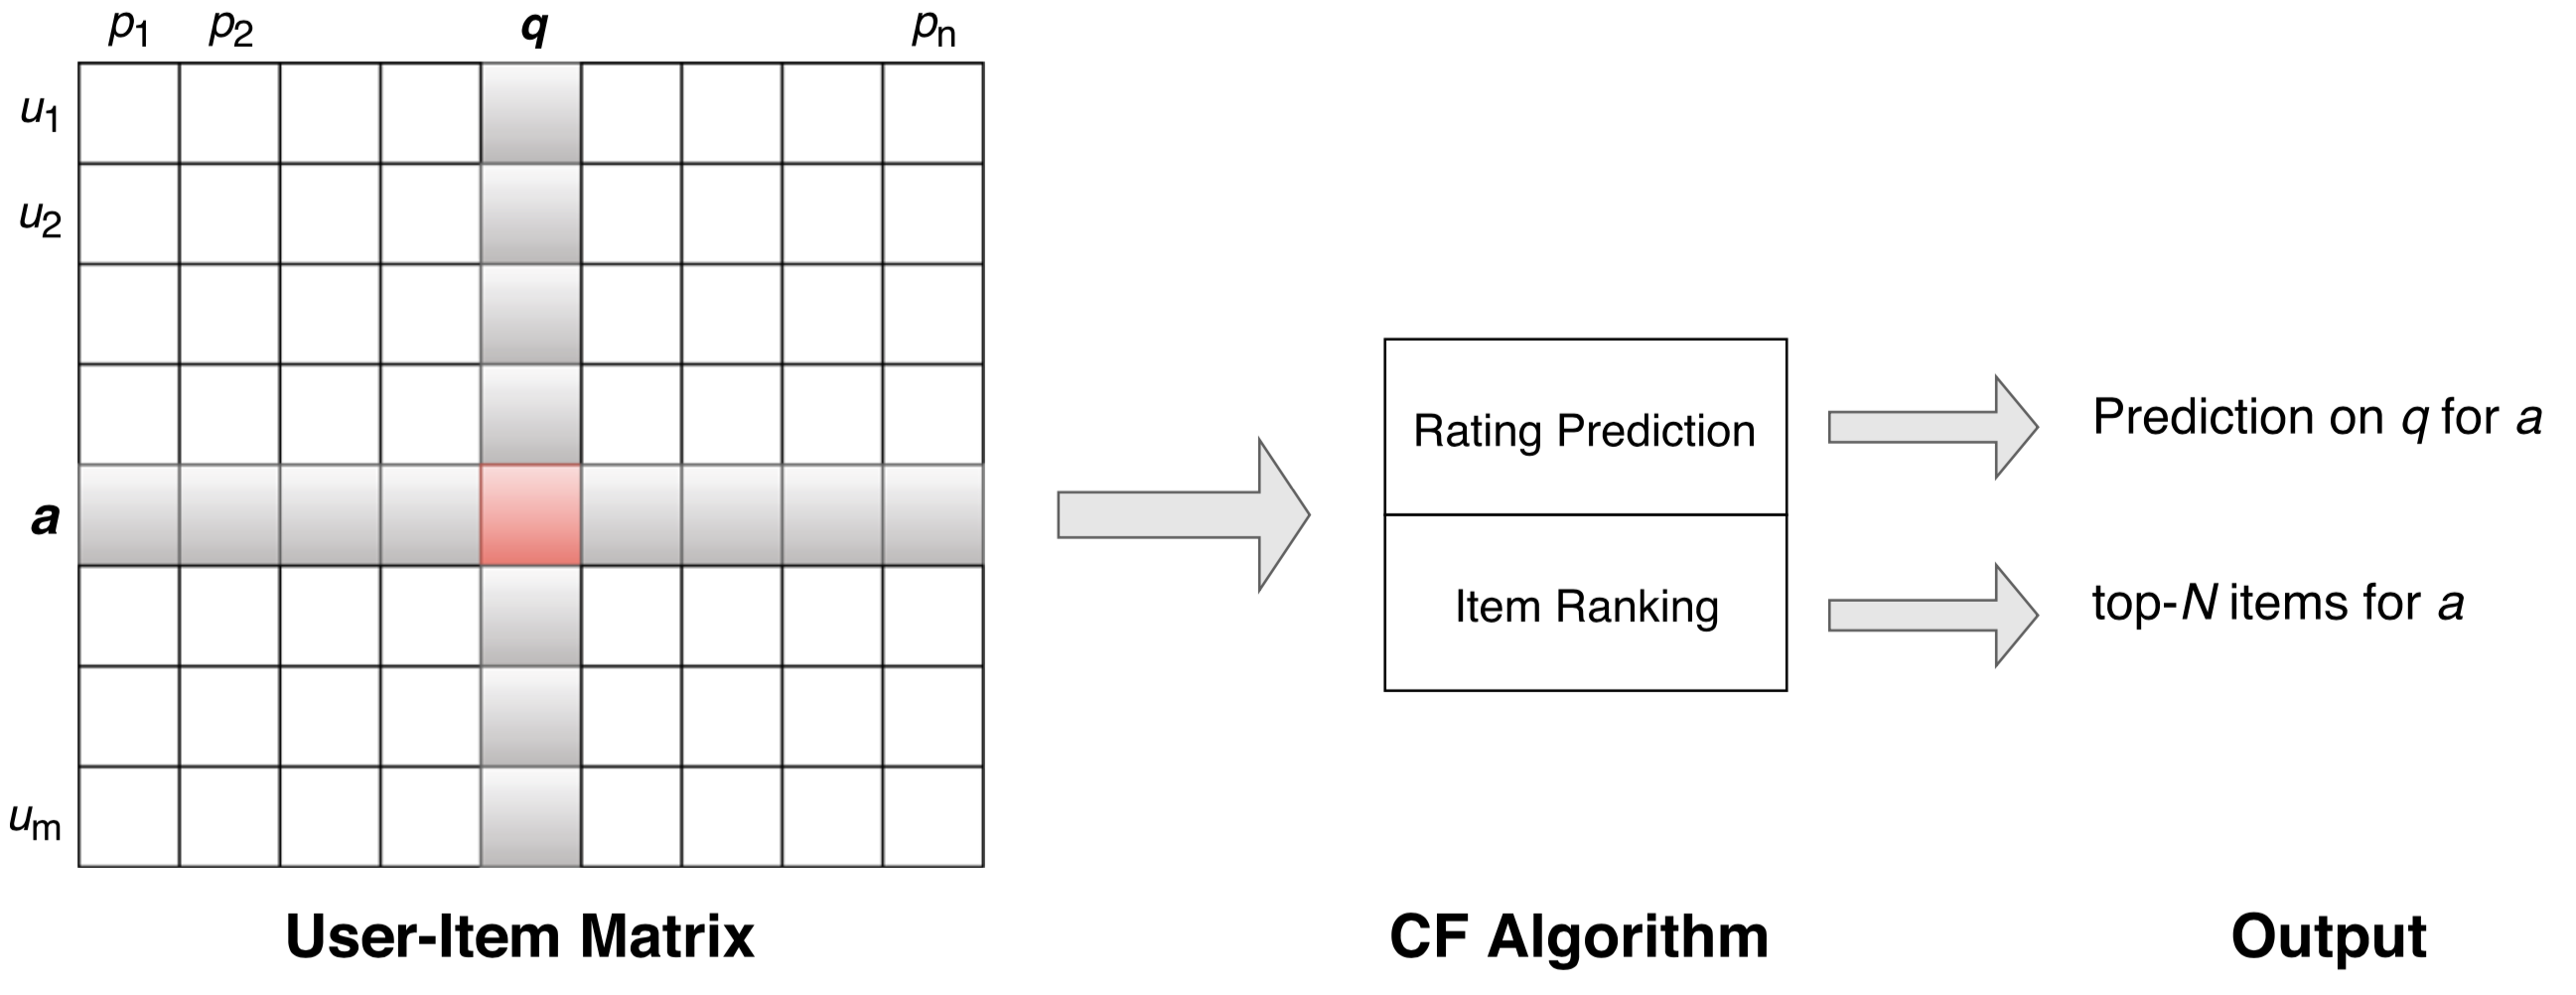
\includegraphics[width=0.9\columnwidth]{CF.png}
	\caption{An overview of the CF process.}
	\label{fig:cf}
	\vspace{-10pt}
\end{figure}
It is important that in such CF systems, preferences of like-minded neighbor 
users form the basis of all produced recommendations rather than individual 
features of items.

Many works \cite{koren2009matrix,salakhutdinov2007probabilistic,yang2012local,zhang2013optimizing} have been proposed based on collaborative filtering.
Among them, latent factor models play a key role in CF methods, ranging from pLSA \cite{hofmann2004latent} and Latent Dirichlet Allocation \cite{blei2003latent} to SVD-based models \cite{koren2008factorization,chen2012svdfeature} and factorization machines \cite{rendle2010factorization}.
% matrix factorization
% neural network for collaborative filtering
Nowadays, deep neural network (DNN) has attracted huge attentions in recommender systems because of its effective feature extraction and end-to-end model training with satisfying generalization \cite{zhang2017deep}.
Some DNN methods \cite{he2017neural,he2018outer,qu2016product} are proposed for latent factor collaborative filtering.
% temporal dynamics for CF-based model
However, almost all of these approaches, either conventional matrix factorization methods or deep models, lack of temporal pattern mining. And the ``collaborative'' part of these models are implicit, though latent factor representation learning.
\cite{koren2009collaborative} firstly proposed a SVD method for temporal dynamics while the model makes several assumptions with hand-engineered temporal bias thus it has poor generalization.
%\cite{wu2017recurrent} utilized RNN for sequence modeling. However, this work does not consider spatial graph information, and the model applis simple sum-pooling of the interacted items in each time slice thus not effective.

We will describe these models in detail in the following subsections:
\subsection{Latent Factor Models}
In this part, we take the famous SVD-based model as an example to describe
the latent factor models.
SVD models are actually a matrix factorization method which map both users 
and items to a joint latent factor space of a low dimension and ratings are
modeled as inner product in that space. Formally, each user $u$ is represented
by a dense vector $p_u \in R^d$ and each item is represented as $q_i \in R^d$
. The rating is calculated as $\hat{r_{ui}} = p_u^T q_i$. To learn the representations
of users and items, we minimize the regularized the squared error:
\begin{equation}
    \min _{q_{*}, p_{*}} \sum_{(u, i, t) \in \mathcal{K}}\left(r_{u i}-q_{i}^{T} p_{u}\right)^{2}+\lambda\left(\left\|q_{i}\right\|^{2}+\left\|p_{u}\right\|^{2}\right).
\end{equation}
This design is not good enough for much of the existed rating values 
are due to effects associated with either users or items, instead of 
their interactions. So bias terms for both user and item are needed in the model.
To achieve this, we use 
\begin{equation}
        \hat{r}_{u i}=\mu+b_{u}+b_{i}+q_{i}^{T} p_{u},
\end{equation}
to calculated the predicted ratings.
Koren et al\cite{koren2008factorization} extended the above model by adding the influence
of the user's interacted items as a feature to the prediction model, as
\begin{equation}
    \hat{r}_{u i}=\mu+b_{i}+b_{u}+q_{i}^{T}\left(p_{u}+|\mathrm{R}(u)|^{-\frac{1}{2}} \sum_{j \in \mathrm{R}(u)} y_{j}\right),
\end{equation}
where the set $R(u)$ contains the items that interacted with user $u$.


\subsection{DNN-based CF Models}
In this section, we present two works that are recently proposed for DNN-based
collaborative filtering recommender.

The first one is NCF \cite{he2017neural} which main contribution is replacing
the inner product with a neural architecture that can learn an arbitrary 
function from data. NCF is generic and can express and generalize matrix 
factorization under its framework.
The formulated framework of NCF is 
\begin{equation}
    \hat{y}_{u i}=f\left(\mathbf{P}^{T} \mathbf{v}_{u}^{U}, \mathbf{Q}^{T} \mathbf{v}_{i}^{I} | \mathbf{P}, \mathbf{Q}, \Theta_{f}\right)
\end{equation}
where $P \in R^{M \times K}$ and $P \in Q^{M \times K}$, denoting the 
latent factor matrix for users and items, respectively; and $\Theta_{f}$
is the parameters set of of the function $f$ which is implemented as a
neural network. Because $f$ is actually a multi-layer perceptron, the 
prediction function can be formulated as
\begin{equation}
    f\left(\mathbf{P}^{T} \mathbf{v}_{u}^{U}, \mathbf{Q}^{T} \mathbf{v}_{i}^{I}\right)=\phi_{o u t}\left(\phi_{X}\left(\ldots \phi_{2}\left(\phi_{1}\left(\mathbf{P}^{T} \mathbf{v}_{u}^{U}, \mathbf{Q}^{T} \mathbf{v}_{i}^{I}\right)\right) \ldots\right)\right).
\end{equation}
The framework is shown in Fig.~\ref{fig:ncf}.
\begin{figure}[h]
	\centering
	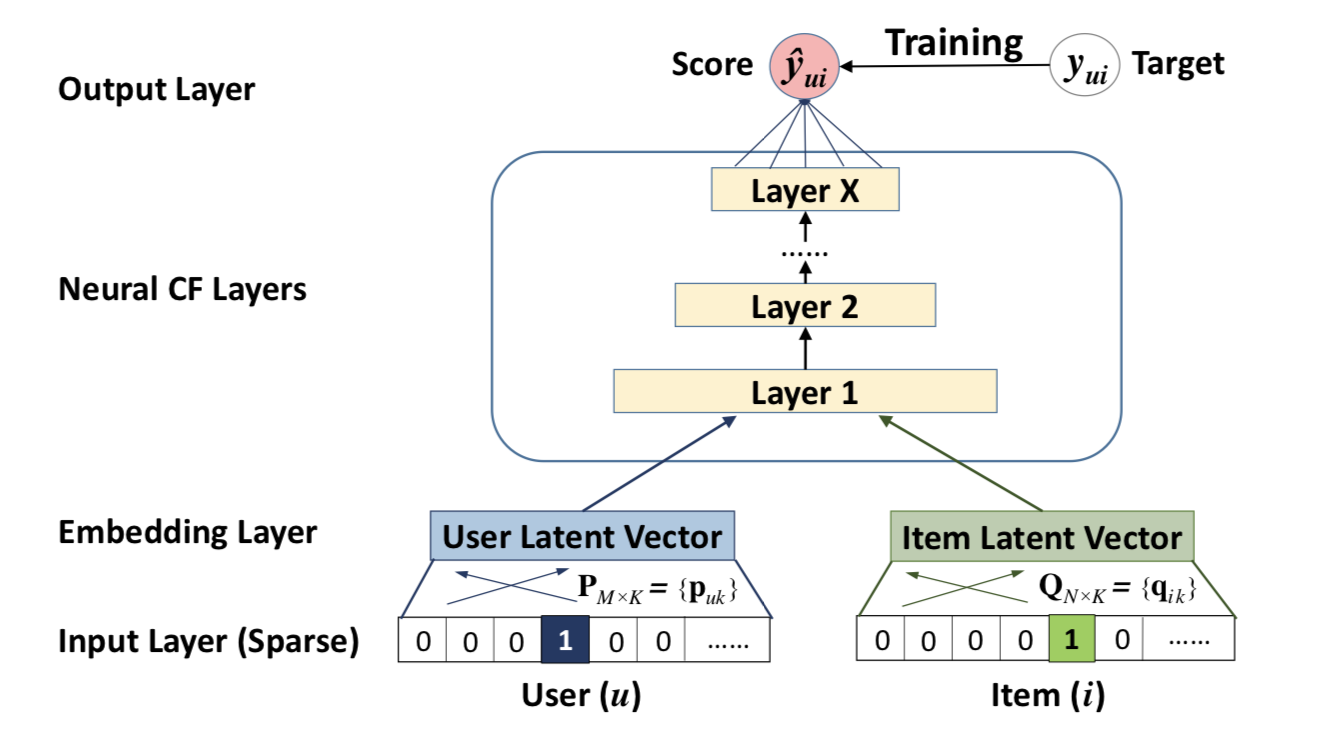
\includegraphics[width=0.9\columnwidth]{NCF.png}
	\caption{Neural collaborative filtering framework.}
	\label{fig:ncf}
	\vspace{-10pt}
\end{figure}
It uses a log-likelihood funciton as the loss function to train the model,
\begin{equation}
    \begin{aligned} L &=-\sum_{(u, i) \in \mathcal{Y}} \log \hat{y}_{u i}-\sum_{(u, j) \in \mathcal{Y}^{-}} \log \left(1-\hat{y}_{u j}\right) \\ &=-\sum_{(u, i) \in \mathcal{Y} \cup \mathcal{Y}^{-}} y_{u i} \log \hat{y}_{u i}+\left(1-y_{u i}\right) \log \left(1-\hat{y}_{u i}\right) \end{aligned}
\end{equation}
whose optimization is done by performing stochastic gradient descent (SGD).

The second one is DELF \cite{cheng2018delf}, a dual-embedding based deep latent factor 
model for recommendation. This model take a dual view from both user-side and
item-side. It not only uses the user's interacted items, but also item's interacted
users. By utilizing dual side information to better model the relationship
between the target user and the target item. Furthermore, DELF employs an 
attention mechanism to discriminate the importance of interacted 
users/items for dual-embedding learning. Another novel attempt of the model 
is modeling the user-item interactions with four deep representations, and a fusion
layer is used to subtly fuse the information of the four representations.
The framework of DELF is shown in Fig. ~\ref{fig:delf}.
\begin{figure}[h]
	\centering
	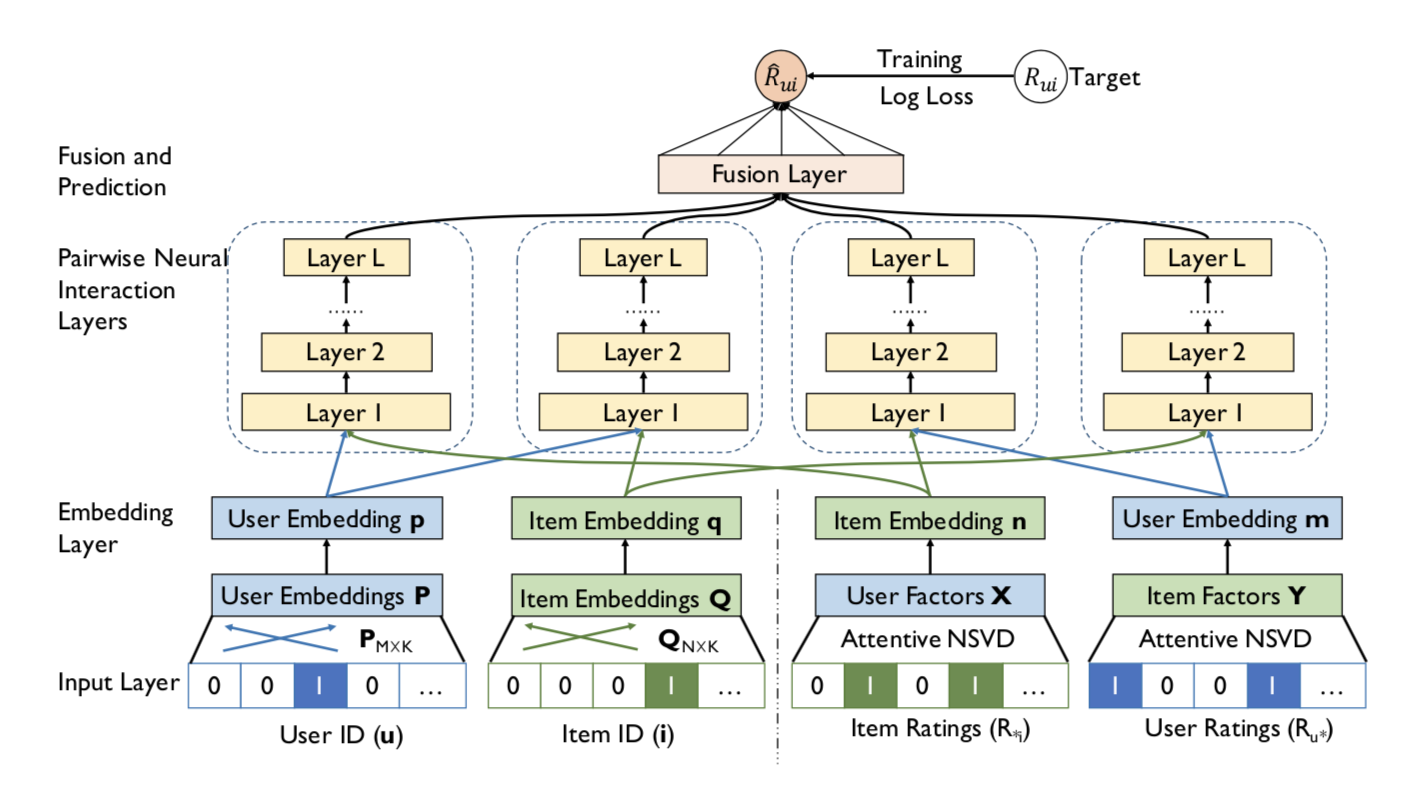
\includegraphics[width=0.9\columnwidth]{DELF.png}
	\caption{DELF framework.}
	\label{fig:delf}
	\vspace{-10pt}
\end{figure}

In this model, the item-based user dense representation $m_u$ is modeled as,
\begin{equation}
    \mathbf{m}_{u}=\sum_{i \in R(u)} \alpha_{i} \mathbf{y}_{i}
\end{equation}
where $\alpha_{i}$ is the attention value which indicates the importance of
the interacted item. The attention value is calculated as,
\begin{equation}
    \begin{aligned} \mathbf{h}_{i} &=\tanh \left(\mathbf{W}_{a} \mathbf{y}_{i}+\mathbf{b}_{a}\right) \\ \alpha_{i} &=\frac{\exp \left(\mathbf{h}_{i}^{T} \mathbf{h}_{a}\right)}{\sum_{i \in R(u)} \exp \left(\mathbf{h}_{i}^{T} \mathbf{h}_{a}\right)} \end{aligned}
\end{equation}
where $W_a$, $b_a$ denote the weight matrix and bias vector respectively, and
$h_a$ is the context vector.
Similarly, it represent the target item with user factors as,
\begin{equation}
    \mathbf{n}_{i}=\sum_{u \in R(i)} \alpha_{u} \mathbf{x}_{u}
\end{equation}
where the users that have interacted with the target item are aggregated as
a user-based item representation. This is the "dual" view of DELF which is 
attentional.

To model the complex feature interactions between $u$ and $i$, DELF uses a 
pairwise neural interaction layer instead of using a single network structure.
It models the user-item interactions in a seperate way, formally,
\begin{equation}
\begin{array}{c}{\mathbf{h}^{j}=\phi_{L}^{j}\left(\ldots \phi_{2}^{j}\left(\phi_{1}^{j}\left(\mathbf{z}_{0}[j]\right)\right) \ldots\right)} \\ {\phi_{l}^{j}=\delta_{l}^{j}\left(\mathbf{W}_{l}^{j} \mathbf{z}_{l-1}^{j}+\mathbf{b}_{l}^{j}\right), l \in[1, L]} \\ {\mathbf{z}_{0}=\left[\mathbf{p}_{u} \oplus \mathbf{n}_{i}, \mathbf{p}_{u} \oplus \mathbf{q}_{i}, \mathbf{m}_{u} \oplus \mathbf{n}_{i}, \mathbf{m}_{u} \oplus \mathbf{q}_{i}\right]}\end{array}
\end{equation}
where $j \in \{1,2,3,4\}$; $h_j$ is the deep representation of embedding representation
which is learned by $j$-th pairwise interaction neural network.
The fusion and prediction layer is defined as,
\begin{equation}
\begin{array}{c}{\mathbf{h}_{f}=\delta_{f}\left(\mathbf{W}_{f} \mathbf{z}_{f}+\mathbf{b}_{f}\right)} \\ {\mathbf{z}_{f}=\mathbf{h}^{1} \oplus \mathbf{h}^{2} \oplus \mathbf{h}^{3} \oplus \mathbf{h}^{4}}\end{array}
\end{equation}
and the prediction function is
\begin{equation}
    \hat{R}_{u i}=\delta_{p}\left(\mathbf{W}_{p} \mathbf{h}_{f}+b_{f}\right)
\end{equation}


\section{Sequential User Modeling}
One key aspect of recommender system is user modeling, i.e. to capture the latent interests of the user and derive the adaptive representation for each user\cite{zhou2018deepa,zheng2017joint}.
Recently, sequential user modeling has drawn huge attention since the sequences of user behaviors have rich information for the user interests, especially for concept drifting \cite{widmer1996learning}, long-term behavior dependency \cite{koren2009collaborative,ren2019lifelong}, periodic patterns \cite{ren2018repeatnet}, etc.

There are three categories for sequential user modeling.
The first one is from the view of temporal collaborative filtering \cite{koren2009collaborative} with the consideration of drifting user preferences.
The second stream is based on Markov-chain methodology \cite{rendle2010factorizing,he2016fusing,he2016vista} which implicitly models the user state dynamics and derive the outcome behaviors.
The third school is based on deep neural networks, such as recurrent neural networks (RNN) \cite{hidasi2015session,hidasi2017recurrent,wu2017recurrent,jing2017neural,liu2016context,beutel2018latent,villatel2018recurrent} and convolutional neural networks (CNN) regarding the behavior history as an image \cite{tang2018personalized,kang2018self}.
However, most of these methods only care about user's interest drifting and do not consider the sequential patterns of items, which also deliver rich information for user-item matching.
Furthermore, most of these sequential models only care about user's own interaction history while ignore the information that could be found in similar users or items.

In the following subsections, we describe the methods of third school using deep neural
networks in details.
\subsection{RNN-based Models}
In this part, we introduce the RNN-based sequential recommendation model. We take
GRU4Rec \cite{hidasi2015session} as an example. This is the first work to use
recurrent neural networks (RNNs) in the domian of recommender system. Real-life 
recommender systems has the problem of having to base recommendations only on 
short term session-based data, instead of long-term user sequential behaviors.
Furthermore, traditional models lack the ability of capturing the sequential 
patterns embedded in the users behaviors.

This model, as indicated by its name: GRU4Rec, utilizes Gated Recurrent Unit to
model the sequential patterns of user behavior. The framework of GRU4Rec is shown
in Fig.~\ref{fig:gru4rec}.
\begin{figure}[h]
	\centering
	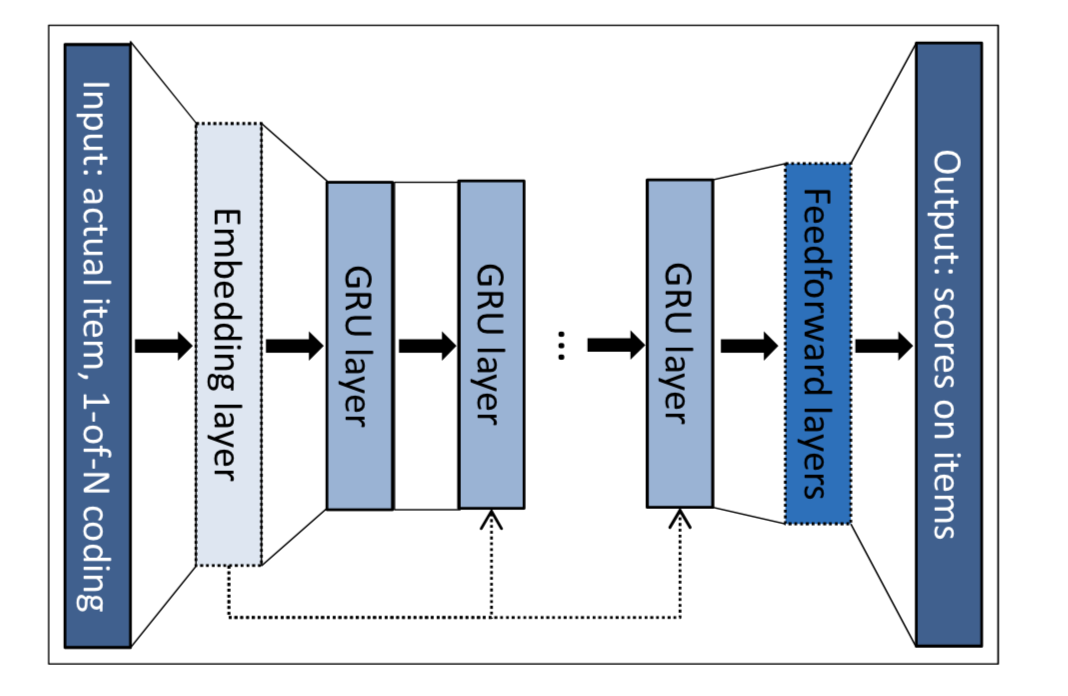
\includegraphics[width=0.8\columnwidth]{GRU4Rec.png}
	\caption{GRU4Rec framework.}
	\label{fig:gru4rec}
	\vspace{-10pt}
\end{figure}
Formally, GRU function is the following, 
\begin{equation}
    \mathbf{h}_{\mathbf{t}}=\left(1-\mathbf{z}_{\mathbf{t}}\right) \mathbf{h}_{\mathbf{t}-\mathbf{1}}+\mathbf{z}_{\mathbf{t}} \hat{\mathbf{h}_{t}}
\end{equation}
where the update gate $\mathbf{z}_t$ is calculated as,
\begin{equation} \label{eq:2-14}
    \mathbf{z}_{\mathbf{t}}=\sigma\left(W_{z} \mathbf{x _ { t }}+U_{z} \mathbf{h}_{\mathbf{t}-\mathbf{1}}\right)
\end{equation}
while the candidate activation function $\hat{\mathbf{h}_t}$ is computed in a similar
manner as, 
\begin{equation}
    \hat{\mathbf{h}_{\mathrm{t}}}=\tanh \left(W \mathbf{x}_{\mathbf{t}}+U\left(\mathbf{r}_{\mathbf{t}} \odot \mathbf{h}_{\mathbf{t}-\mathbf{1}}\right)\right)
\end{equation}
and the final reset gate $\mathbf{r}_t$ is given by,
\begin{equation}
    \mathbf{r}_{\mathbf{t}}=\sigma\left(W_{r} \mathbf{x}_{\mathbf{t}}+U_{r} \mathbf{h}_{\mathbf{t}-\mathbf{1}}\right)
\end{equation}
In Eq.~\ref{eq:2-14}, $\mathbf{x}_t$ is the input, which is the user behavior at
each time which is actually item that is clicked by the user. It is notable that
we use one-hot encoding to represent the items, and they need to be fed to
an embedding layer first before the GRU layers, as shown in Fig.~\ref{fig:gru4rec}.

GRU4Rec uses \textbf{BPR} (Bayesian Personalized Ranking) ranking loss, 
which is defined as,
\begin{equation}
    L_s = -\frac{1}{N_{S}} \cdot \sum_{j=1}^{N_{S}} \log \left(\sigma\left(\hat{r}_{s, i}-\hat{r}_{s, j}\right)\right)
\end{equation}
It compares the score of a positive and a sampled negative item, and tries
to maximize the score of the positive item while minimize the score of the negative
sample.

\subsection{CNN-based Models}
In this subsection, we introduce the CNN-based sequential recommender system: Caser
\cite{tang2018personalized}. The main idea of this model is to regard the user
sequential behaviors as an image by embedding the user's recent interacted items
into low-dimension representations. And it is the first work to utilize convolutional
neural networks (CNNs) in the domain of sequential user modeling. CNNs achieve
huge success in computer vision field, and this work shows that it has its
protential in sequential pattern mining and its time complexity is better than
the RNN-based models.

The Caser framework is shown in Fig.~\ref{fig:caser}
\begin{figure}[h]
	\centering
	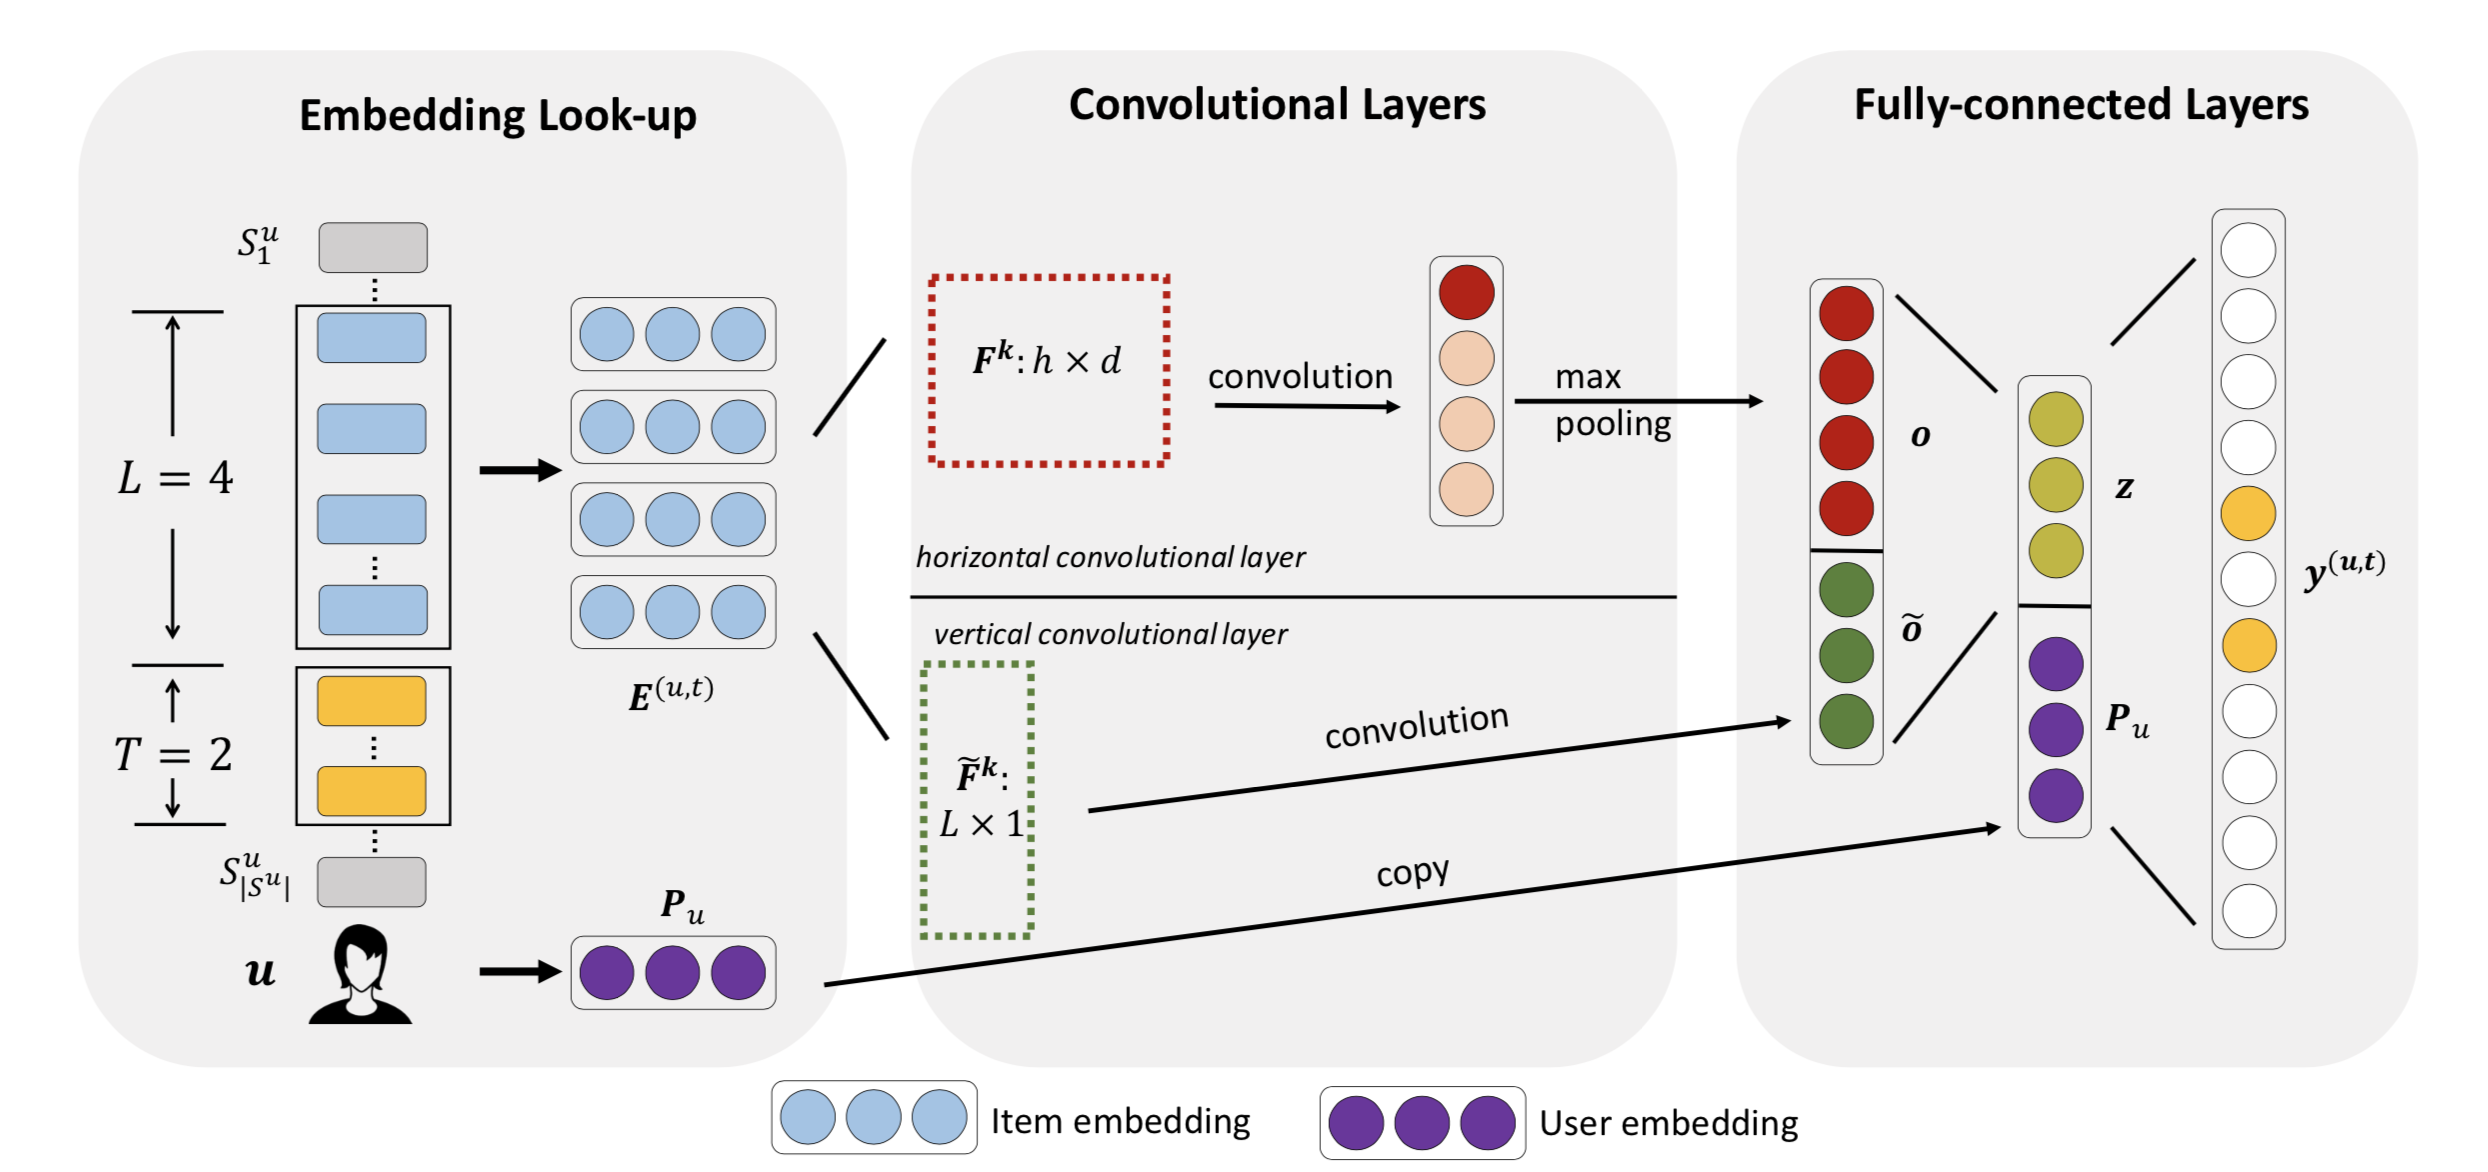
\includegraphics[width=0.9\columnwidth]{Caser.png}
	\caption{Caser framework.}
	\label{fig:caser}
	\vspace{-10pt}
\end{figure}
it uses convolution kernels as the sequential pattern aggregators. Caser
convolves from both horizontal and vertical directions.
The network is trained with \textit{cross-entropy} loss.
\begin{equation}
    \ell=\sum_{u} \sum_{t \in C^{u}} \sum_{i \in \mathcal{D}_{t}^{u}}-\log \left(\sigma\left(\boldsymbol{y}_{i}^{(u, t)}\right)\right)+\sum_{j \neq i}-\log \left(1-\sigma\left(\boldsymbol{y}_{j}^{(u, t)}\right)\right)
\end{equation}

\subsection{Attention-based Models}
In this subsection, we describe the newly emerging attention-based models for 
sequential user modeling. SASRec \cite{kang2018self} is based on Transformer \cite{vaswani2017attention},
which utilizes self-attention mechanism to capture sequential patterns.
The key part of SASRec is the multi-head self-attention block, which is defined as,
\begin{equation}
    \text { Attention }(\mathbf{Q}, \mathbf{K}, \mathbf{V})=\operatorname{softmax}\left(\frac{\mathbf{Q} \mathbf{K}^{T}}{\sqrt{d}}\right) \mathbf{V}
\end{equation}
where $Q$ is the queries, $K$ the keys and $V$ the values. "Self-"attention means
that $Q = K = V$. Formally defined as,
\begin{equation}
    \mathbf{S}=\mathrm{SA}(\widehat{\mathbf{E}})=\text { Attention }\left(\widehat{\mathbf{E}} \mathbf{W}^{Q}, \widehat{\mathbf{E}} \mathbf{W}^{K}, \widehat{\mathbf{E}} \mathbf{W}^{V}\right)
\end{equation}
This process can be reproduced multiple times, thus it forms the multi-head
self-attention block.
Though the self-attention is able to aggregate all previous items’ 
embeddings with adaptive weights, but it is still a linear model. To give it 
non-linear abilities to capture more complex patterns, it defines a point-wide
feed-forward network as, 
\begin{equation}
    \mathbf{F}_{i}=\mathrm{FFN}\left(\mathbf{S}_{i}\right)=\operatorname{ReLU}\left(\mathbf{S}_{i} \mathbf{W}^{(1)}+\mathbf{b}^{(1)}\right) \mathbf{W}^{(2)}+\mathbf{b}^{(2)}
\end{equation}
Thus, the multi-head self-attention mechanism is conducted through stacking
self-attention blocks as, 
\begin{equation}
\begin{array}{c}{\mathbf{S}^{(b)}=\mathrm{SA}\left(\mathbf{F}^{(b-1)}\right)} \\ {\mathbf{F}_{i}^{(b)}=\mathrm{FFN}\left(\mathbf{S}_{i}^{(b)}\right), \quad \forall i \in\{1,2, \ldots, n\}}\end{array}
\end{equation}
The model is trained using \textit{cross-entropy loss}. It is important that
SASRec uses more supervision signals at each time point, which is shown in Fig.~\ref{fig:sasrec}.
\begin{figure}[h]
	\centering
	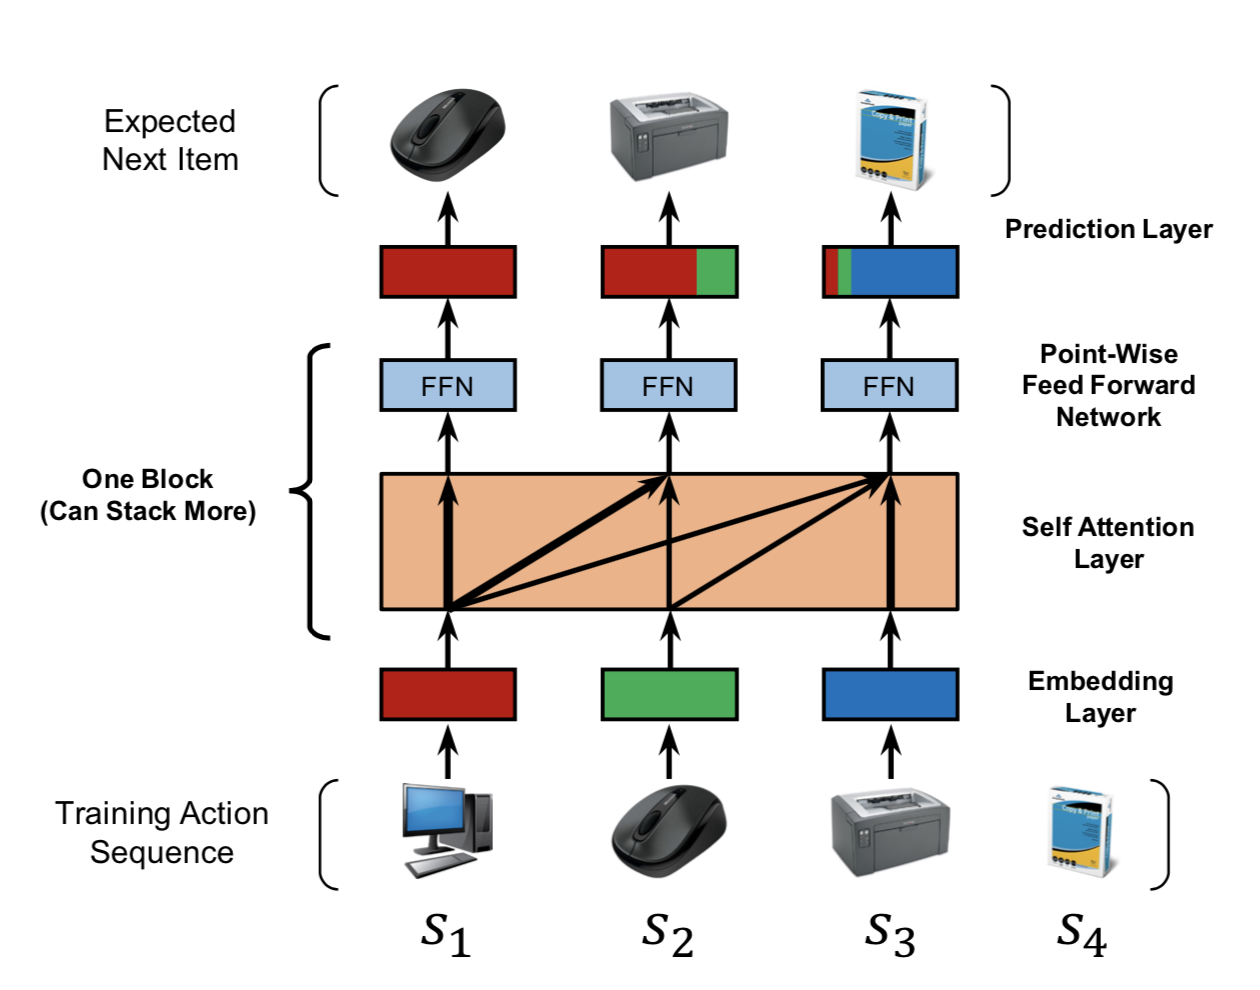
\includegraphics[width=0.8\columnwidth]{SASRec.png}
	\caption{A simplified diagram showing the training process of SASRec.}
	\label{fig:sasrec}
	\vspace{-10pt}
\end{figure}
At each time step, the model considers all previous items, and uses attention to ‘focus on’ items relevant to the next action.
Another significant part of SASRec is the position embedding that makes each position has its
own low-dimension vector representation. Position embeddings are used to provide
sequential information for the model, because SASRec is not an auto-regressive model.
So, the embedding matirx $\widehat{\mathbf{E}}$ is defined as,
\begin{equation}
\widehat{\mathbf{E}}=\left[ \begin{array}{c}{\mathbf{M}_{s_{1}}+\mathbf{P}_{1}} \\ {\mathbf{M}_{s_{2}}+\mathbf{P}_{2}} \\ {\cdots} \\ {\mathbf{M}_{s_{n}}+\mathbf{P}_{n}}\end{array}\right]
\end{equation}

\section{Graph Pattern Mining in Recommender Systems}
In the domain of recommender systems, there are two schools of graph pattern mining methods.

The first school of models make use of additional information such as social networks \cite{song2019session,wu2019dual} or knowledge graphs \cite{wang2018ripplenet} to enhance the learning process of user-user relations or item-item relations respectively. These models are tricky since they use other side information which may not be easy to obtain.

The second school only uses user-item bipartite interaction graph.
The perspective of bipartite graph is novel for recommender system \cite{fadel2018link}, which could be facilitated by the recent advances of graph pattern mining \cite{kipf2016semi} and link prediction in graph domain \cite{van2017graph}.
\cite{niu2018collaborative} utilize the graph information of both the target user and the target item for better collaborative filtering while they ignore the temporal dynamics of the evolving graphs.
\cite{wu2017recurrent} use RNNs to do sequence modeling for both user and item side. However, the model applies simple sum-pooling on the interacted items/users in each time slice thus not effective.
The model proposed in \cite{fadel2018link} captures spatial graph patterns along timeline with graph convolutional networks (GCN) \cite{van2017graph}. However, they just consider the first-order relations without collaborative information among the graphs.

In the following subsections, we describe the methods of the two schools in details.

\subsection{Social Network-based Models}
Social Network is a good source to get user-user relationships. It is an important
assumption that friends are more likely to have similar tastes, so the opinions
of friends plays an important role in the decision making process of the 
target user.

We introduce the state-of-the-art model in social sequential recommendation,
DGRec \cite{song2019session} which is shown in Fig.~\ref{fig:dgrec}.
\begin{figure}[h]
	\centering
	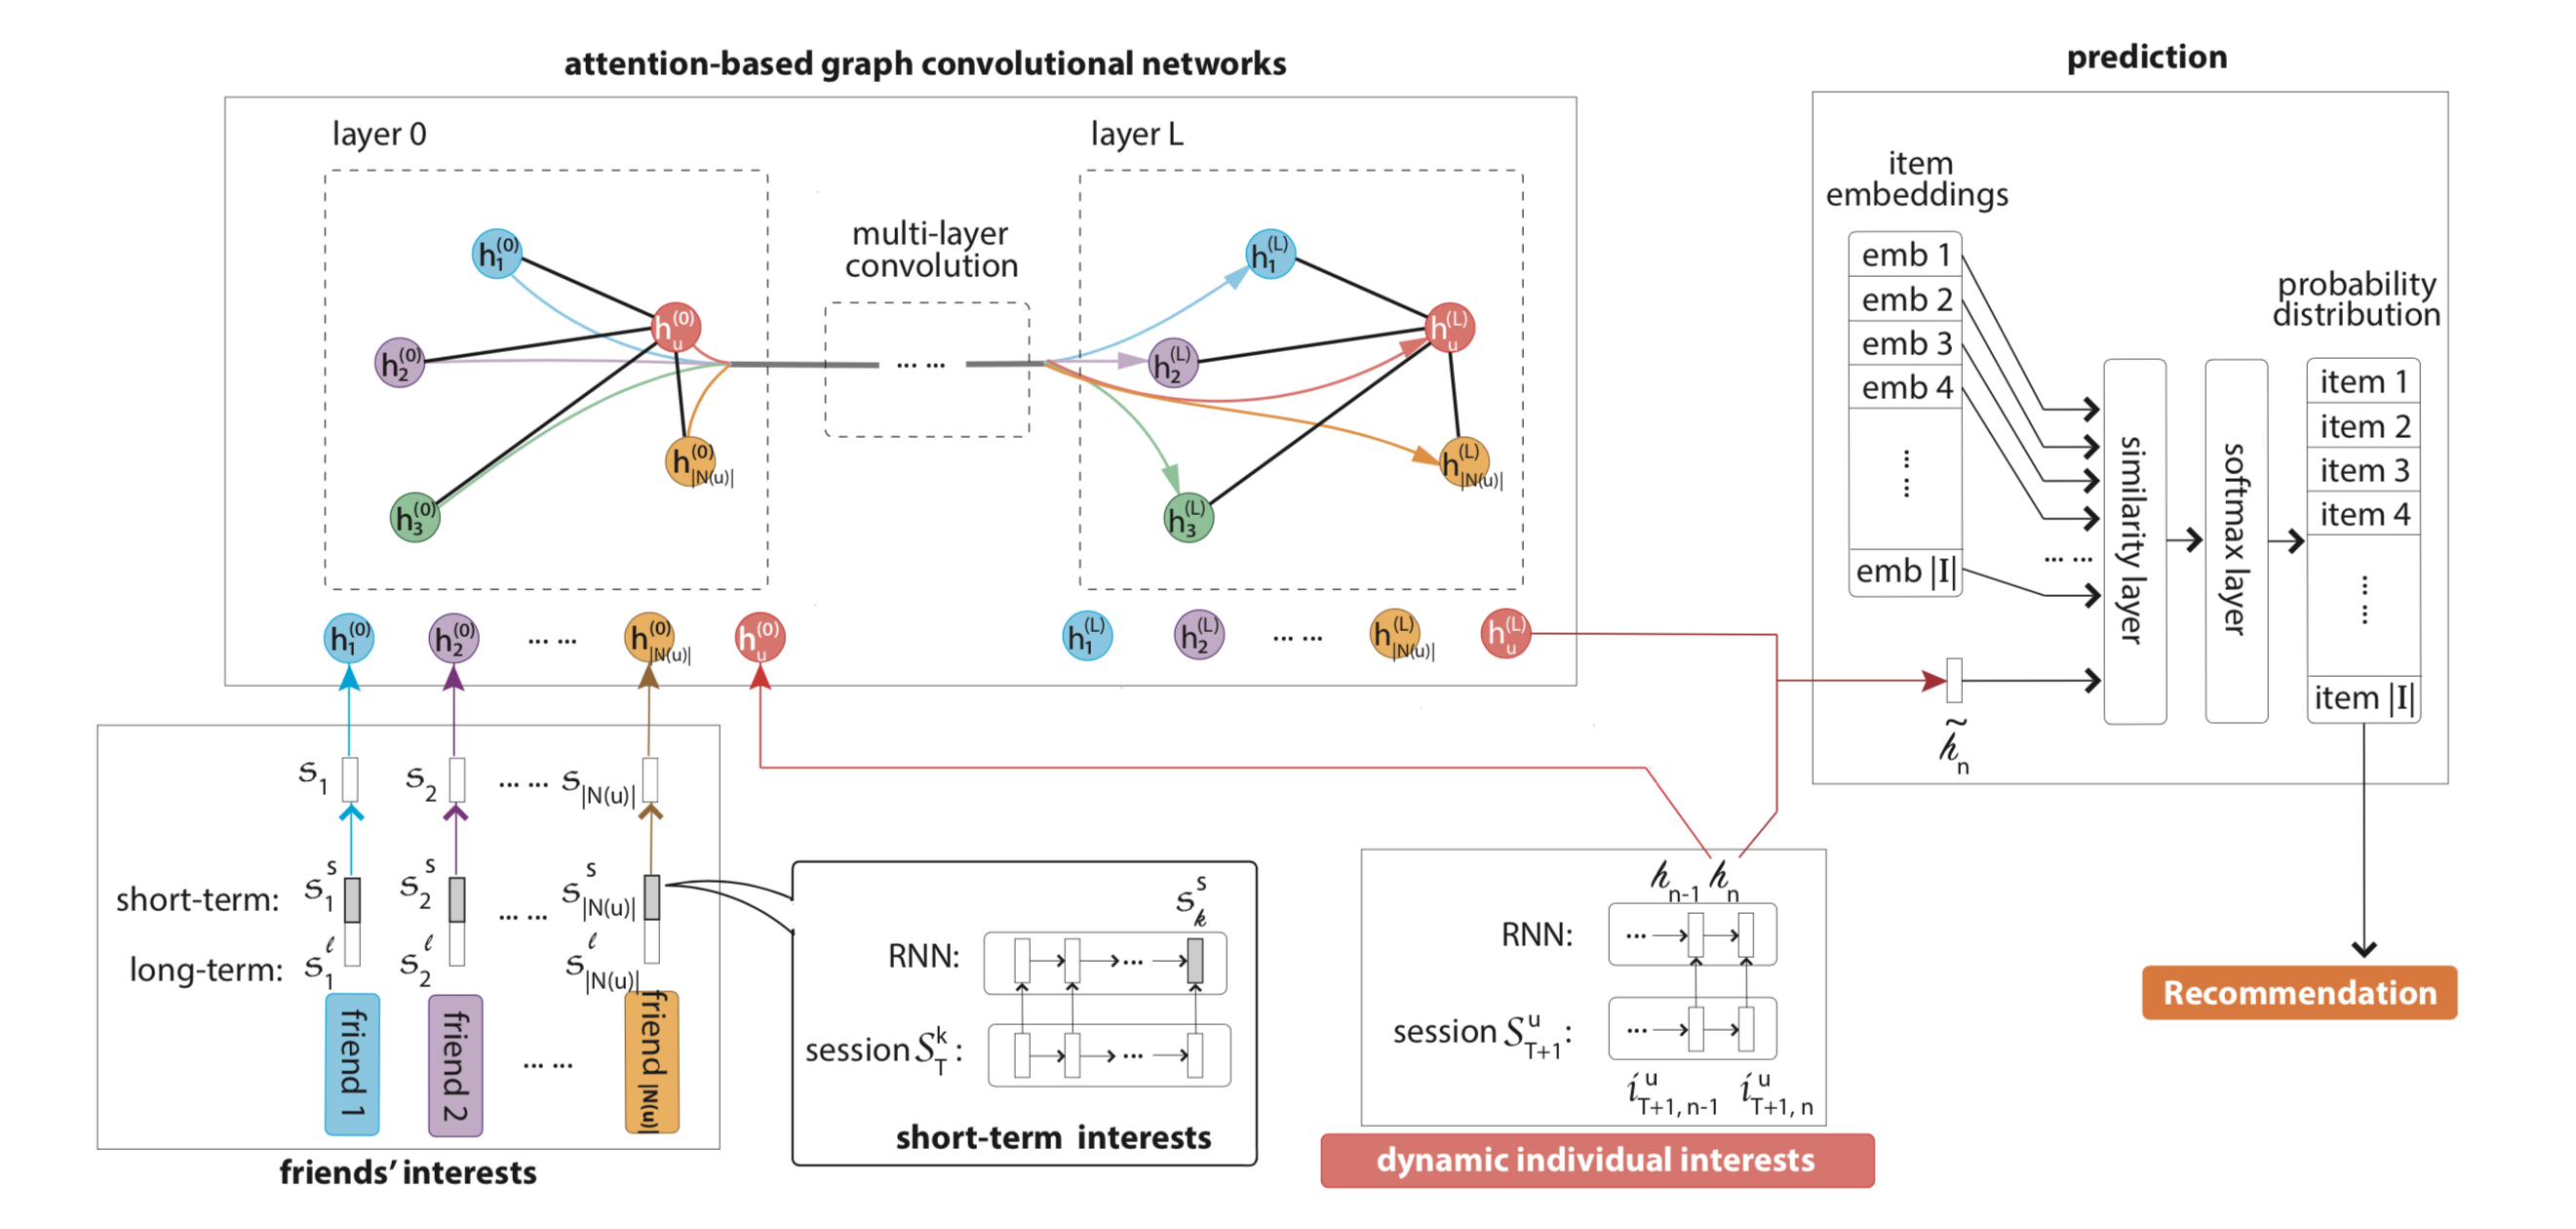
\includegraphics[width=1.0\columnwidth]{DGRec.png}
	\caption{A schematic view of DGRec for dynamic social recommendation.}
	\label{fig:dgrec}
	\vspace{-10pt}
\end{figure}
DGRec uses RNN to model the short-term user interest dynamics as,
\begin{equation}
    h_{n}=f\left(i_{T+1, n}^{u}, h_{n-1}\right)
\end{equation}
where $h_n$ represents the user's interests and $f(\cdot, \cdot)$ is a non-linear
funciton combining both sources of information. In practice, $f$ is modeled
by Long Short-Term Memory (LSTM) as,
\begin{equation}
\begin{aligned} x_{n} &=\sigma\left(\mathbf{W}_{x}\left[h_{n-1}, i_{T+1, n}^{u}\right]+b_{x}\right) \\ f_{n} &=\sigma\left(\mathbf{W}_{f}\left[h_{n-1}, i_{T+1, n}^{u}\right]+b_{f}\right) \\ o_{n} &=\sigma\left(\mathbf{W}_{o}\left[h_{n-1}, i_{T+1, n}^{u}\right]+b_{o}\right) \\ \tilde{c}_{n} &=\tanh \left(\mathbf{W}_{c}\left[h_{n-1}, i_{T+1, n}^{u}\right]+b_{c}\right) \\ c_{n} &=f_{n} \odot c_{n-1}+x_{n} \odot \tilde{c}_{n} \\ h_{n} &=o_{n} \odot \tanh \left(c_{n}\right) \end{aligned}
\end{equation}
where $\sigma$ is the sigmoid funciton: $\sigma(x)=(1+\exp (-x))^{-1}$.

The target user is represented by its short-term interest which is used as 
the context of recommendation. And the long-term representation is just from
a embedding matrix.

DGRec uses Graph Attention Network to aggregate the friends' interests.
It calculates the similarity between the target user's node 
representation $h_u^{(l)}$ and all of its neighbors' representations $h_k^{(l)}$:
\begin{equation}
    \alpha_{u k}^{(l)}=\frac{\exp \left(f\left(h_{u}^{(l)}, h_{k}^{(l)}\right)\right)}{\sum_{j \in N(u) \cup\{u\}} \exp \left(f\left(h_{u}^{(l)}, h_{j}^{(l)}\right)\right)}
\end{equation}
where $h_u^{(l)}$ is the representation of the target user at layer $l$, and
$f\left(h_{u}^{(l)}, h_{k}^{(l)}\right)=h_{u}^{(l)^{\top}} h_{k}^{(l)}$ is the 
similarity function between two elements. So, the final representation of the 
target user node is 
\begin{equation}
    \tilde{h}_{u}^{(l)}=\sum_{k \in N(u) \cup\{u\}} \alpha_{u k}^{(l)} h_{k}^{(l)}
\end{equation}
which is used in the prediction function.

\subsection{Knowledge Graph-based Models}
In this section, we introduce RippleNet \cite{wang2018ripplenet} which is proposed
to use knowledge graph information to enhance the performance of recommendation.
Similar to actual ripples propagating on the water, RippleNet stimulates 
the propagation of user interests over the set of entities in the KG
by iteratively and automatically extending a user’s potential interests 
along links in the KG. The multiple "ripples" activated by 
a user’s historically clicked items are thus superposed to form the 
preference distribution of the user with respect to a candidate item, 
which could be used for predicting the final clicking probability.
The framework of RippleNet is shown in Fig.~\ref{fig:ripplenet}.
\begin{figure}[h]
	\centering
	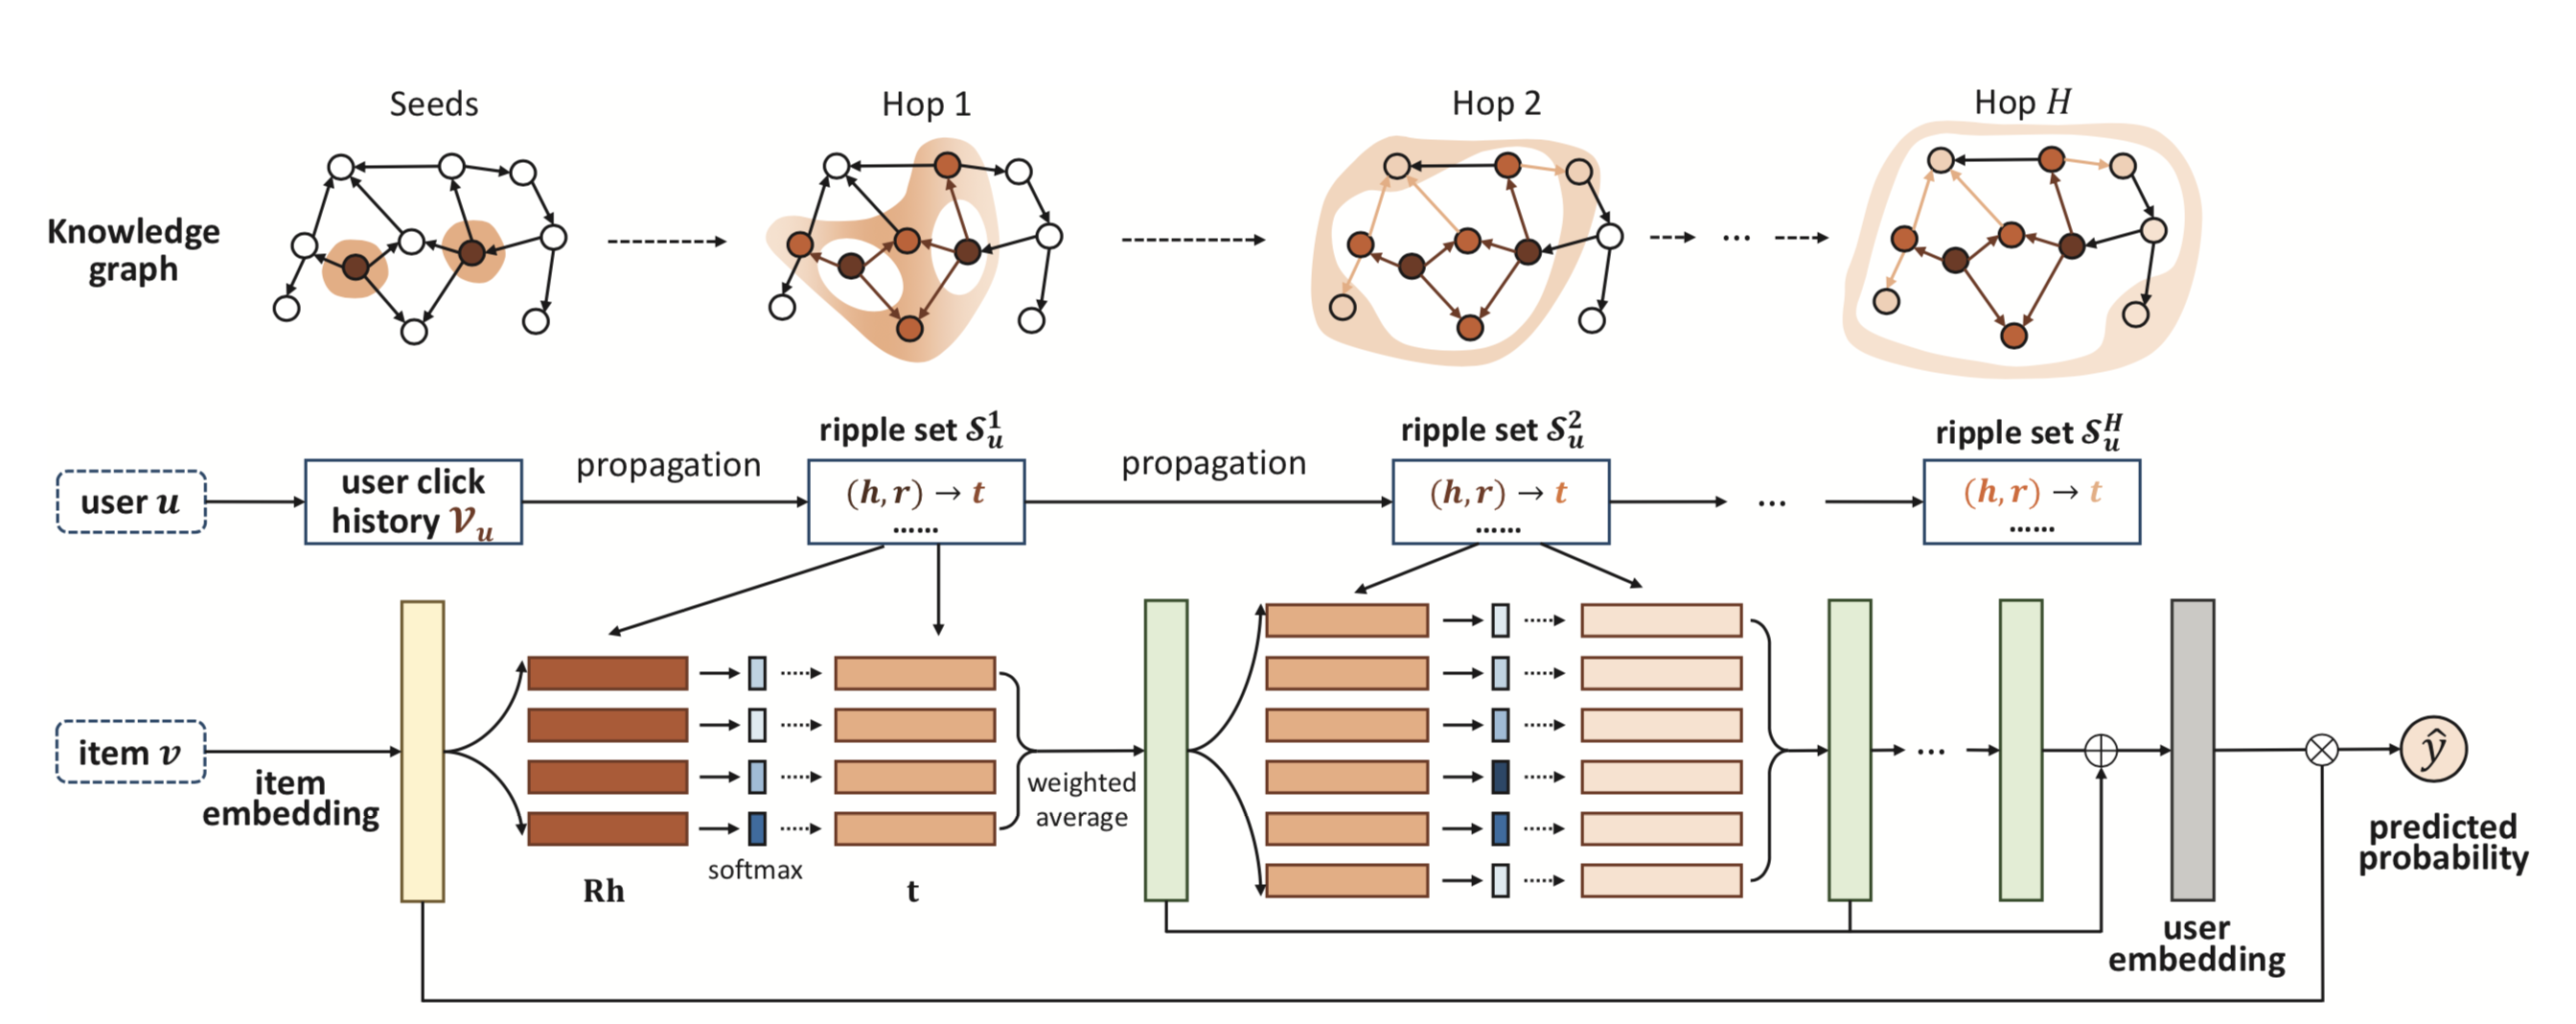
\includegraphics[width=1.0\columnwidth]{RippleNet.png}
	\caption{The overall framework of the RippleNet.}
	\label{fig:ripplenet}
	\vspace{-10pt}
\end{figure}

At each hop, the items in the ripple set is weighted by an attention mechanism utilizing
the KG information as,
\begin{equation}
    p_{i}=\operatorname{softmax}\left(\mathbf{v}^{\mathrm{T}} \mathbf{R}_{i} \mathbf{h}_{i}\right)=\frac{\exp \left(\mathbf{v}^{\mathrm{T}} \mathbf{R}_{i} \mathbf{h}_{i}\right)}{\sum_{(h, r, t) \in \mathcal{S}_{u}^{1}} \exp \left(\mathbf{v}^{\mathrm{T}} \mathbf{R} \mathbf{h}\right)}
\end{equation}
where $R_i \in R^{d \times d}$ and $h_i \in R^d$ are the embeddings of relation
$r_i$ and head $h_i$ respectively, and $\mathbf{v}$ is the item embedding in the
ripple set.
Thus, the user representation is given by 
\begin{equation}
    \mathbf{u}=\mathbf{o}_{u}^{1}+\mathbf{o}_{u}^{2}+\ldots+\mathbf{o}_{u}^{H},    
\end{equation}
and the final prediction score is $\hat{y}_{u v}=\sigma\left(\mathbf{u}^{\mathrm{T}} \mathbf{v}\right)$,
where $\sigma(x)=\frac{1}{1+\exp (-x)}$ is the sigmoid funciton. And the model
is trained by minimizing negative log likelihood as, 
\begin{equation}
\begin{aligned} \min \mathcal{L}=&-\log (p(\mathrm{Y} | \Theta, \mathcal{G}) \cdot p(\mathcal{G} | \Theta) \cdot p(\Theta)) \\=& \sum_{(u, v) \in \mathrm{Y}}-\left(y_{u v} \log \sigma\left(\mathbf{u}^{\mathrm{T}} \mathbf{v}\right)+\left(1-y_{u v}\right) \log \left(1-\sigma\left(\mathbf{u}^{\mathrm{T}} \mathbf{v}\right)\right)\right) \\ &+\frac{\lambda_{2}}{2} \sum_{r \in \mathcal{R}}\left\|\mathbf{I}_{r}-\mathbf{E}^{\mathrm{T}} \mathbf{R E}\right\|_{2}^{2}+\frac{\lambda_{1}}{2}\left(\|\mathbf{V}\|_{2}^{2}+\|\mathbf{E}\|_{2}^{2}+\sum_{r \in \mathcal{R}}\|\mathbf{R}\|_{2}^{2}\right) \end{aligned}
\end{equation}

\subsection{User-item Bipartite Graph-based Models}
In this part, we introduce two models which are based on user-item bipartite
graphs to do sequential modeling. 

\begin{figure}[h]
	\centering
	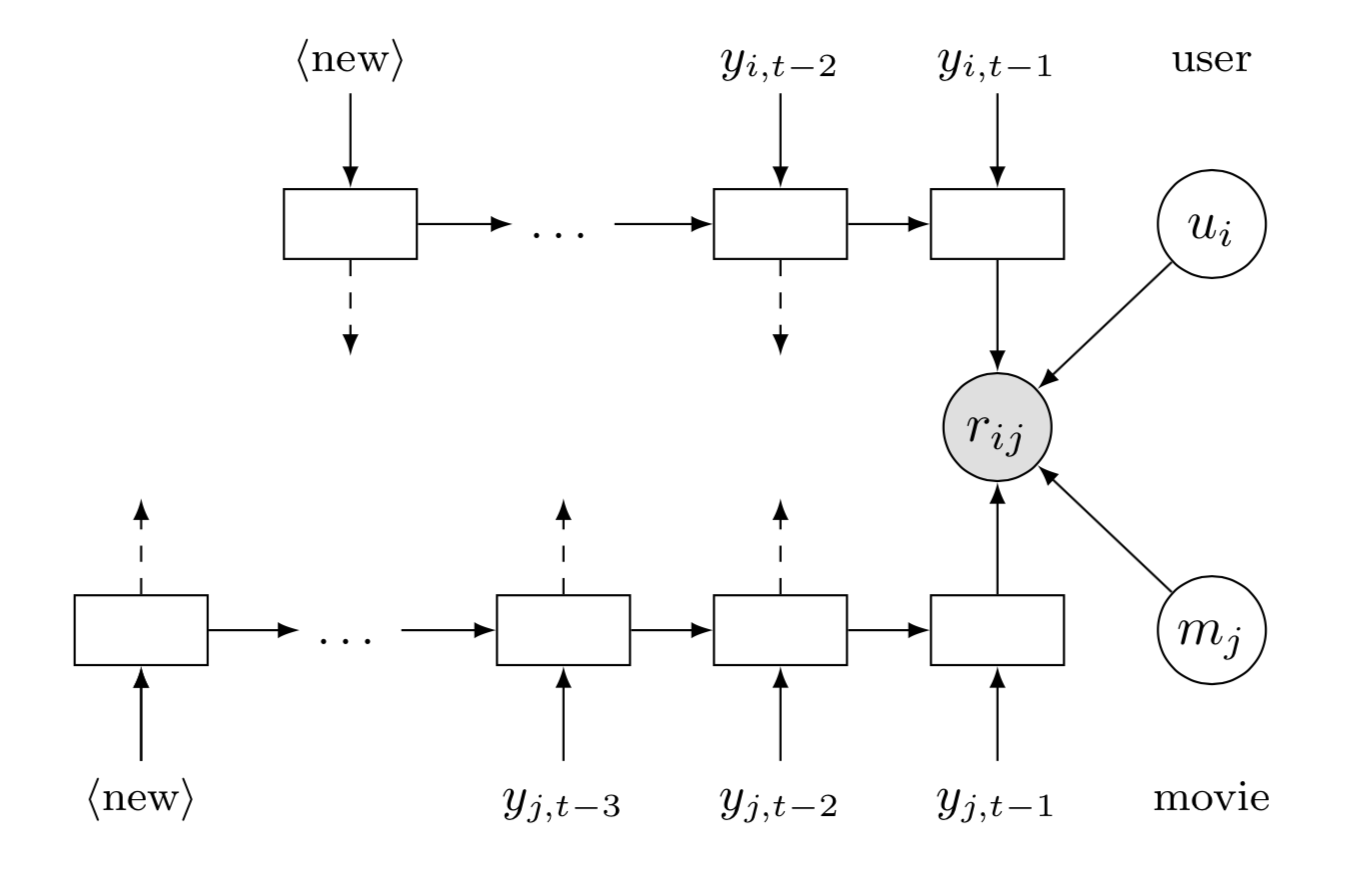
\includegraphics[width=0.8\columnwidth]{RRN.png}
	\caption{The overall framework of the RRN.}
	\label{fig:rrn}
	\vspace{-10pt}
\end{figure}

The first one is RRN \cite{wu2017recurrent}. It is a dual-sequence model which
uses both the user and item-side temporal dynamics. RRN can be regard as a
graph model, for it uses the first-order neighbor of the target user and item.
The framework of RRN is shown in Fig.~\ref{fig:rrn}

It splits the timeline into $T$ slices, and in each time slice, RRN uses
sum pooling as the graph information aggregator as,
\begin{equation}
    y_{t} :=W_{\text { embed }}\left[x_{t}, 1_{\text { newbie }}, \tau_{t}, \tau_{t-1}\right]
\end{equation}
where $x_t$ is a multi-hot embedding indicating the items/users that are
interacted by the target user/item. And the temporal dynamics are modeled using
LSTM as $u_{t} :=\operatorname{LSTM}\left(u_{t-1}, y_{t}\right)$.
Thus, the prediction function is 
\begin{equation}
    \hat{r}_{i j | t}=f\left(u_{i t}, m_{j t}, u_{i}, m_{j}\right) :=\left\langle\tilde{u}_{i t}, \tilde{m}_{j t}\right\rangle+\left\langle u_{i}, m_{j}\right\rangle
\end{equation}
where $\tilde{u}_{i t}$ is calculated as,
\begin{equation}
    \tilde{u}_{i t}=W_{\mathrm{user}} u_{i t}+b_{\mathrm{user}} \text { and } \tilde{m}_{j t}=W_{\mathrm{movie}} m_{j t}+b_{\mathrm{movie}}.
\end{equation}
The model is trained through optimizing the squared error.


The second model is GCMC \cite{fadel2018link} which models the sequential
recommendation task as a dynamic graph link prediction problem. It uses Graph
Convolution Network (GCN) to aggregate the graph information and uses RNN
to capture the sequential pattern of streaming graphs. This model also splits
the timeline into $T$ slices.

The framework of GCMC is shown in Fig.~\ref{fig:gcmc}.

\begin{figure}[h]
	\centering
	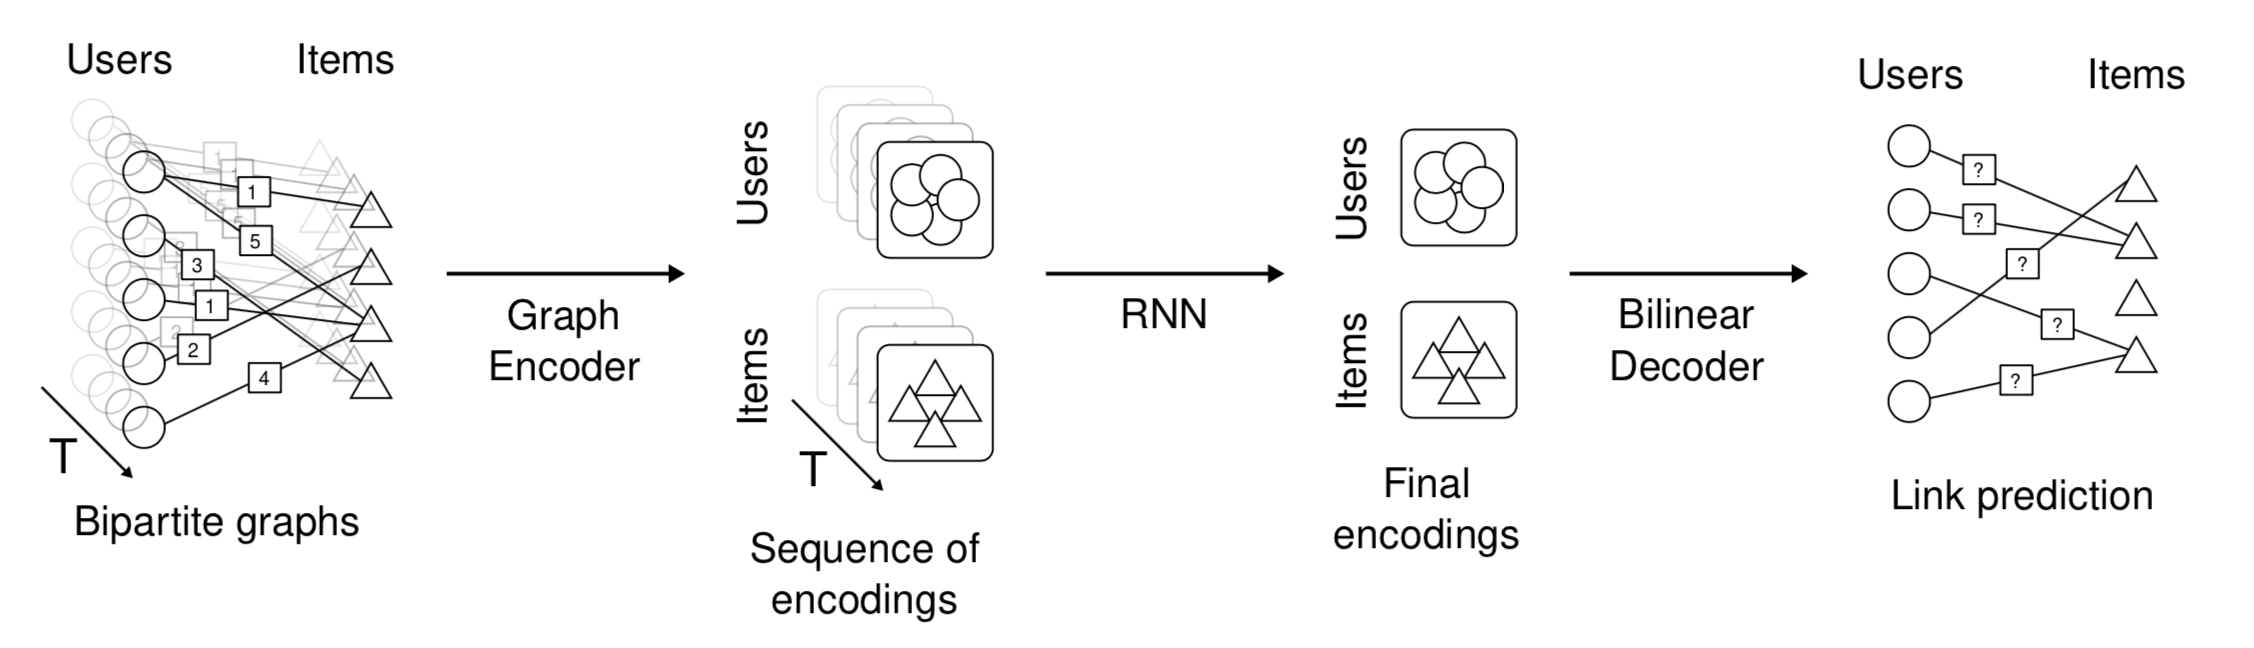
\includegraphics[width=1.0\columnwidth]{GCMC.png}
	\caption{The overall framework of the GCMC.}
	\label{fig:gcmc}
	\vspace{-10pt}
\end{figure}

It uses a GCN-like graph aggregator called Graph Convolution Matrix Completion,
which is defined as,
\begin{equation}
\left.\begin{array}{c}{\mathbf{h}_{u_{i}}=\xi\left(\operatorname{accum}_{r \in \mathcal{R}}\left\{\sum_{j \in \mathcal{N}_{i, r}} \frac{1}{c_{i j}} W_{r} \mathbf{x}_{v_{j}}\right\}\right)} \\ {\mathbf{z}_{u_{i}}=\xi\left(W \mathbf{h}_{u_{i}}\right)}\end{array}\right\}
\end{equation}
where $N_{i, r}$ is the neighbor set of the target user/item, $c_{ij}$ is a normalization constant,
$\operatorname{accum}(\cdot)$ denotes an accumulation function that 
can be either a vector concatenation or sum operation. And $\xi$ is the non-linear
activation function.

Then, the prediction of the score is given by,
\begin{equation}
    P\left(\hat{M}_{i j}=r\right)=\frac{\exp \left(\mathbf{z}_{u_{i}}^{T} Q_{r} \mathbf{z}_{v_{j}}\right)}{\sum_{s \in \mathcal{R}} \exp \left(\mathbf{z}_{u_{i}}^{T} Q_{s} \mathbf{z}_{v_{j}}\right)}
\end{equation}
where each $Q_r \in R^{d_{output} \times d_{output}}, r \in R$ is learned during training process.
The model is trained to minimize the negative logarithmic likelihood of 
the predicted ratings as,
\begin{equation}
    \mathcal{L}(M, \hat{M})=-\sum_{\left(u_{i}, r, v_{j}\right) \in \mathcal{E}} \log P\left(\hat{M}_{i j}=r\right).
\end{equation}
